\documentclass[a4paper,12pt]{article}
\setlength{\oddsidemargin}{0mm}
\setlength{\textwidth}{16.8cm}
\setlength{\topmargin}{0mm}
\setlength{\textheight}{23cm}
\setlength{\headsep}{0in}
\setlength{\headheight}{0pt}
\pagestyle{plain}

%\usepackage[dvips]{graphics}   % unix environment
%\usepackage[textures]{graphics}  % mac textures environment
\usepackage{url,amsmath}

\usepackage{color}
%\usepackage{pslatex}
%\usepackage[dvips,draft]{graphicx}   % unix environment
\usepackage[dvips,final]{graphicx}   % unix environment

\usepackage{amsmath}
\usepackage{hyperref}

\DeclareGraphicsExtensions{.jpg,.eps}
\DeclareGraphicsRule{.jpg}{eps}{.jpg.bb}{`jpeg2ps -h -r 600 #1}
\graphicspath{{Figures/}{eps/}}

\definecolor{blue}{rgb}{0,0,1} % blue
\definecolor{bluegreen}{rgb}{0,0.5,0.5} % blue green
\definecolor{redblue}{rgb}{0.5,0,0.5} % red blue

% Each section have independent equation numbering like (2.12)
%\def\theequation{\arabic{section}.\arabic{equation}}
%\def\thefigure{\arabic{section}.\arabic{figure}}
\newtheorem{exercise}{Exercise}
\newtheorem{theorem}{Theorem}
%\newtheorem{lemma}[theorem]{Lemma}             % the same numbering as theorem
%\newtheorem{proposition}[theorem]{Proposition} % the same numbering as theorem
%\newtheorem{corollary}[theorem]{Corollary}     % the same numbering as theorem
%\newtheorem{property}[theorem]{Property}       % the same numbering as theorem
%\newtheorem{remark}[theorem]{Remark}           % the same numbering as theorem
%\newtheorem{assumption}[theorem]{Assumption}   % the same numbering as theorem

\newcommand{\Hrule}{\noindent \hrulefill}
\newcommand{\HBrule}{\noindent \hrulefill \medskip}
\newcommand{\HTrule}{\medskip \noindent \hrulefill}

\def\mbzero{\mbox{\boldmath$0$}}
\def\dim{\mathop{\it dim}\nolimits}
\def\conv{\mathop{\it conv}\nolimits}
\def\cone{\mathop{\it cone}\nolimits}
\def\aff{\mathop{\it aff}\nolimits}
\def\lin{\mathop{\it lin}\nolimits}
\def\linsp{\mathop{\it lin.space}\nolimits}
\def\chcone{\mathop{\it char.cone}\nolimits}
\newcommand{\FL}[1]{\left\lfloor #1  \right\rfloor}
\newcommand{\RF}[1]{\left\lceil #1  \right\rceil}


%\psdraft
\title
{Frequently Asked Questions in Polyhedral Computation}

\author
{{Komei Fukuda}\\
   ETH Zurich, Switzerland\\
    fukuda@math.ethz.ch\\
    \url{https://people.inf.ethz.ch/fukudak/}
}

\date{Version Jan 15, 2022}

\begin{document}

\maketitle

\begin{center}
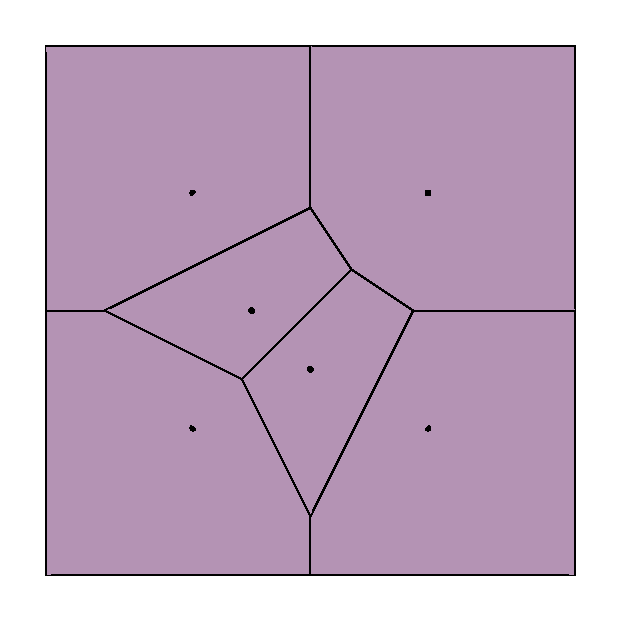
\includegraphics[height=40mm]{vtest_fig_vo.eps}
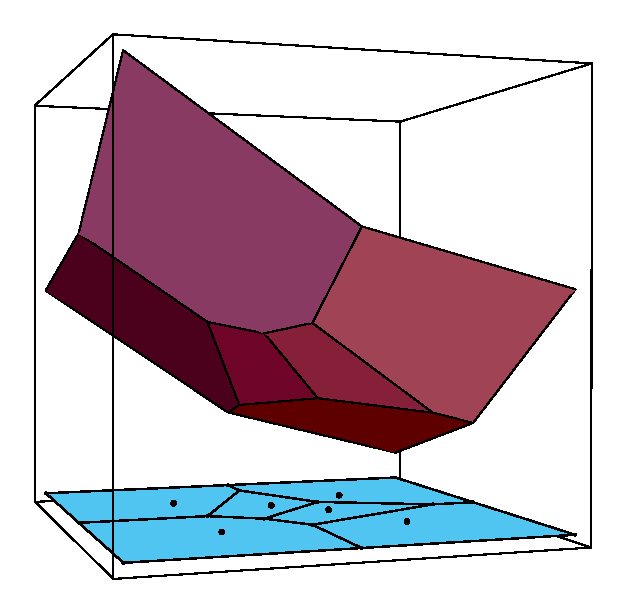
\includegraphics[height=40mm]{vtest_fig_vo3d.eps}
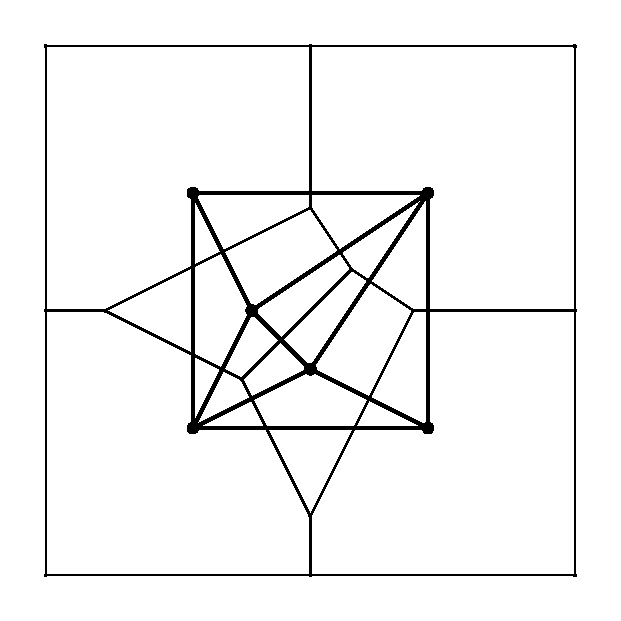
\includegraphics[height=40mm]{vtest_fig_vode.eps}
\end{center}

\tableofcontents


% --------------------- Introduction --------------------------------------
\section{What is Polyhedral Computation FAQ?}  \label{Sec:intro}

This is an FAQ to answer some basic questions arising from
certain geometric computation in general dimensional 
(mostly Euclidean) space.   The main areas to be covered
are the convex hull computation of a finite point set, 
the vertex enumeration for a convex polytope,
the computation of Voronoi diagram and Delaunay triangulation, in $R^d$.
We illustrate typical solution processes with small examples and
publicly available codes such as cddlib \cite{f-cddhome}  and lrslib \cite{a-lrshome-01}.

It is still incomplete and perhaps contains a number of
typos and mistakes at this moment, but I will try to
make it as complete as possible for the primary purposes.

We do not intend to discuss techniques and algorithms
specially designed for particular dimensions (e.g. 2D and 3D).
For those interested primarily in geometric computation in
lower dimensions (e.g. 2 and 3) should consult the
 comp.graphics.algorithms {FAQ}
 \cite{o-cgafaq} as well as a handbook of discrete and 
computational geometry \cite{go-hbdcg-97}.

Please note that the Polyhedral Computation FAQ is available from 
\cite{f-kfhome} in pdf format. The html version might become
available as well, and it has an advantage of having
html links within the documents.  Yet, one has to be aware of
the fact that some conversion errors exist that give 
wrong equation numberings and
missing figures.  Please consider the pdf version as the most reliable source.

We do not provide any proofs for the stated results in this document.
 The basic theory and computational algorithms on convex polyhedra are presented
with rigorous proofs in the textbook \cite{f-pc-20}.

To refer to this document, please use
\begin{quote}
Komei Fukuda\\
Polyhedral computation {FAQ}\\
 ETH Zurich, Switzerland\\
    fukuda@math.ethz.ch\\
\url{https://people.inf.ethz.ch/fukudak/}.
\end{quote}
Please send your comments to the email address above.
% --------------------- Polyhedron --------------------------------------
\section{Convex Polyhedron}  \label{Sec:polytope}
\subsection{What is convex polytope/polyhedron?} \label{polytope:polytope}

A subset $P$ of $R^d$ is called a {\em convex polyhedron\/} if it is
the set of solutions to a finite system of linear inequalities, and 
called {\em convex polytope\/} if it is a convex polyhedron and bounded.
When a convex polyhedron (or polytope) has dimension $k$, it is
called a {\em $k$-polyhedron\/} ({\em $k$-polytope\/}).
For the sequel, we might omit  {\bf convex} for convex polytopes
and polyhedra, and call them simply polytopes and polyhedra.

\subsection{What are the faces of a convex polytope/polyhedron?} \label{polytope:faces}

Let $P$ be a convex $d$-polyhedron (or $d$-polytope) in $R^d$.

For a real $d$-vector $c$ and a real number $d$, a linear inequality 
$c^T x \le d$ 
is called {\em valid\/} for $P$ if $c^T x \le d$ holds for all $x \in P$.
A subset $F$ of a polyhedron $P$ is called a {\em face\/} of $P$ if it is
represented as
\[
   F= P \cap \{ x:  c^Tx = d \}
\]
for some valid inequality $c^T x \le d$.  By this definition,
both the empty set $\emptyset$ and the whole set $P$ are
faces.  These two faces are called {\em improper\/} faces while the other
faces are called {\em proper\/} faces.

We can define faces geometrically.  For this, we need to
define the notion of supporting hyperplanes. 
A hyperplane $h$ of $R^d$ is {\em supporting
$P$\/} if one of the two closed halfspaces of $h$ contains $P$.   
A subset $F$ of $P$ is called a {\em face\/} of $P$ 
if it is either $\emptyset$, $P$
itself or the intersection of $P$ with a supporting hyperplane.

The faces of dimension $0$, $1$, $\dim(P)-2$ and $\dim(P)-1$ are called the {\em vertices\/},
{\em edges\/}, {\em ridges\/} and {\em facets\/}, respectively.  
The vertices coincide
with the {\em extreme points\/} of $P$ which are defined as points which cannot
be represented as convex combinations of two other points in $P$.
When an edge is not bounded, there are two cases: either it is a line
or a half-line starting from a vertex.  
A half-line edge is called an {\em extreme ray\/}.

\subsection{What is the face lattice of a convex polytope}
\label{polytope:facelattice}

The {\em face poset\/} $FL(P)$ of a convex polyhedron is 
the set of all faces of $P$ ordered by set inclusion.
Two polytopes are called {\em isomorphic\/} if
their face posets are isomorphic.  
The face poset of a convex polytope is a lattice.

The face poset of a convex polyhedron is sometimes
referred to as the {\em combinatorial structure\/} of the polyhedron.
Thus the expression ``two polyhedra are combinatorially equal''
means they are isomorphic.

\subsection{What is a dual of a convex polytope?} \label{polytope:dual}

For a convex polytope $P$, any convex polytope $P'$ with $FL(P')$
anti-isomorphic to $FL(P)$ (i.e. ``upside-down'' of $FL(P)$)
is called a {\em (combinatorial) dual\/} of $P$.  By the definition,
a dual polytope has the same dimension as $P$. The duality theorem
states that every convex polytope admits a dual.

\begin{theorem} [Duality of Polytopes] \label{thm:polydual}
Every nonempty $d$-polytope $P$ in $R^d$ 
admits a dual polytope in $R^d$.  In particular,
one can construct a dual polytope by the following ``polar'' construction:
\[
  P^* = \{y \in R^d:  x^T y \le 1 \text{ for all } x \in P \}
\]
where $P$ is assumed to contain the origin in its interior.
\end{theorem}

When $P$ contains the origin in its interior,
the polytope $P^*$ is called the {\em polar\/} of $P$.   One can
easily show that
\[
  P^* = \{y \in R^d:  v^T y \le 1 \text{ for all } v \in  V(P) \}
\]
where $V(P)$ denote the set of vertices of $V$, and this inequality
(H-) representation of $P^*$ is minimal (i.e. contains 
no redundant inequalities).

\subsection{What is simplex?} \label{polytope:simplex}

A subset $P$ of $R^d$ is called a {\em $k$-simplex\/} ($k =0,1, 2, \ldots$)
if it is the convex hull of $k+1$ affinely independent points. It has
exactly $k+1$ vertices and $k+1$ facets.   A simplex is
a $k$-simplex for some $k$.

Simplices are selfdual, i.e. a dual (see \ref{polytope:dual}) of a simplex is again a simplex.

\subsection{What is cube/hypercube/cross polytope?} \label{polytope:hypercube}

A subset $P$ of $R^d$ is called a {\em unit $d$-cube\/} if it is
the convex hull of all $2^d$ points with components $0$ or $1$.   It has
exactly $2^d$ vertices and $2 d$ facets.  A {\em cube\/} or 
{\em hypercube\/} is a 
convex polytope which is isomorphic to the $d$-cube for some
$d$.

A dual (see \ref{polytope:dual}) of a cube is called
a {\em cross\/} polytope.

\subsection{What is simple/simplicial polytope?} \label{polytope:simpsimp}

A $d$-polytope is called {\bf simple} if each vertex is contained
in exactly $d$ facets.   A $d$-polytope is called {\bf simplicial} 
if each facet contains exactly $d$ vertices.  By definition,
a dual of simple (simlicial)
polytope is simplicial (simple, respectively).
Every facet of a simplicial $d$-polytope is a $(d-1)$-simplex.  Each vertex
of a simple $d$-polytope is contained in exactly $d$-edges.

A $d$-cube is a simple polytope and a $d$-simplex is both simple and
simplicial.

\subsection{What is 0-1 polytope?} \label{polytope:01}

A polytope in $R^d$ is called {\bf 0-1} if all its vertices
are in $\{0, 1\}^d$.  In other words, a 0-1 polytope is 
the convex hull of a subset of the $2^d$ point set $\{0, 1\}^d$,
for some $d\ge 0$.

\subsection{What is the best upper bound of the numbers of 
$k$-dimensional faces of a $d$-polytope with $n$ vertices?} \label{polytope:upperbound}

Let $f_k(P)$ denote the number of $k$-faces of a $d$-polytope $P$,
for $k=0,1,\ldots,d$.

The exact upper bound for $f_k$ in terms of $f_0$ and $d$.
is known, thanks to McMullen's upper bound theorem.

The convex hull of distinct $n$ points on the moment curve
$\{m(t)=(t^1, t^2, \ldots, t^d) : t\in R \}$ in $R^d$
is known as a {\em cyclic polytope}.   It is known that
its combinatorial structure (i.e. its face lattice, see 
Section \ref{polytope:facelattice})
 is uniquely determined by $n$ and $d$.
Thus we often write $C(d, n)$ to denote any such
cyclic $d$-polytope with $n$ vertices.

McMullen's Upper Bound Theorem shows that the maximum
of $f_k(P)$ is attained by the cyclic polytopes.
 
\begin{theorem} [Upper Bound Theorem] \label{thm:MUB}
For any $d$-polytope with $n$ vertices,  
\[
  f_k(P)  \le f_{k}(C(d,n)),  \; \forall k=1, \ldots, d-1,
\]
holds.
\end{theorem}

The number of $k$-faces of a cyclic polytope $C(d,n)$ can
be explicitely given and thus one can evaluate the order of
the upper bound in terms of $n$ and $d$.

\begin{theorem} \label{thm:Cyclic}
For $d \ge 2$ and $0 \le k \le d-1$,
\[
 f_{k}(C(d,n)) = \sum_{r=0}^{\lfloor d/2 \rfloor}
\binom{n-d+r-1}{r} \binom{r}{k}
+
\sum_{r=\lfloor d/2 \rfloor+1}^{d}
\binom{n-r-1}{d-r} \binom{r}{k} .
\]  In particular,
\begin{align} \label{polytope:FacetUB}
 f_{d-1}(C(d,n))  
  &= \binom{n-\RF{d/2}}{\left\lfloor \frac{d}{2} \right\rfloor} + \binom{n-\FL{d/2}-1}{\left\lceil \frac{d}{2} \right\rceil -1}\\
   & = O(n^{\left\lfloor \frac{d}{2} \right\rfloor}) \text{\quad for any fixed $d$}.
\end{align}
\end{theorem}


\noindent
For example,

\[
\begin{array}{lrrrrr}
P       & f_0 &  f_1 & f_2 &  f_3 & f_4 \\  
C(5,10) &  10  &  45 &   100 &   105  &  42\\
C(5,20) &  20  & 190 &   580 &   680  & 272\\
C(5,30) &  30  & 435 &  1460 &  1755  & 702
\end{array}
\]

The upper bound theorem can be written in dual  form which
gives, for example, the maximum number of vertices in
a $d$-polytope with $m$ facets.

\begin{theorem} [Upper Bound Theorem in Dual Form] \label{thm:MUBDual}
For any $d$-polytope with $m$ facets,  
\[
  f_k(P)  \le f_{d-k-1}(C(d,m)),  \; \forall k=0,1, \ldots, d-2,
\]
holds.
\end{theorem}


The original proof of the Upper Bound Theorem is in
\cite{m-mnfcp-70,ms-cpuc-71}.
There are different variations, 
see \cite{k-lpsasp-97,m-cg-94,z-lop-94}.  The textbook \cite[Chap 6]{f-pc-20} 
presents a detailed proof based on \cite{k-lpsasp-97} which is beautiful 
but has a little typo.

\subsection{What is convex hull?  What is the convex hull problem?}
\label{polytope:convhullcomp}

For a subset $S$ of $R^d$, the convex hull $conv(S)$ is defined
as the smallest convex set in $R^d$ containing $S$.

The convex hull computation means the ``determination''
of $conv(S)$ for a given finite set of $n$ points 
$S =  \{p^1, p^2, \ldots, p^n\}$
in $R^d$.  

The usual way to determine $conv(S)$ is to
represent it as the intersection of halfspaces, or more precisely,
as a set of solutions to a minimal system of linear inequalities.
This amounts to output a matrix $A \in R^{m \times d}$ and
a vector $b\in R^m$ for some $m$ such that 
$conv(S) =\{ x | A \; x \le b \}$.
When $conv(S)$ is full-dimensional, 
each (nonredundant) inequality corresponds to
a facet of $conv(S)$.  Thus the convex hull problem is
also known as the {\em facet enumeration problem}, see 
Section \ref{polytope:repconv}.

Some people define the convex hull computation as the determination
of extreme points of $conv(S)$, or equivalently that of
redundant points in $S$ to determine $conv(S)$.  This is much simpler
computation than our convex hull problem.  In fact, this can be done
by solving $O(n)$ linear programs and thus polynomially solvable, 
see Section \ref{polytope:Vredundancy}
and \ref{polytope:Vredundancy2}.
It is better to name this as the ``redundancy removal for a point set $S$''.

\subsection{What is the Minkowski-Weyl theorem for convex polyhedra?
 } 
\label{polytope:MWtheorem}

The Minkowski-Weyl Theorem states every polyhedron is
finitely generated and every finitely generated set is a
polyhedron.  More precisely,
for two subsets $P$ and $Q$ of $R^d$, $P+Q$ denotes the
{\em Minkowski sum} of $P$ and $Q$:
\begin{eqnarray*}
    P + Q & = & 
    \{ p +q: p \in P \mbox{ and } q \in Q  \}.
\end{eqnarray*}

\begin{theorem} [Minkowski-Weyl's Theorem] \label{thm:Minkowski-Weyl1}
For a subset $P$ of $R^d$, the  following statements are equivalent:
\begin{description}
\item[(a)] P is a polyhedron, i.e., for some real (finite) matrix $A$ and real vector $b$,
$ P=\{ x :  A  x  \le  b \}$;

\item[(b)] There are finite real vectors $v_1, v_2, \ldots, v_n$ and 
$r_1, r_2, \ldots, r_s$ in $R^d$
such that\\
$P = conv(v_1, v_2, \ldots, v_n) + nonneg(r_1, r_2, \ldots, r_s)$. 
\end{description}
\end{theorem}

Thus, every polyhedron has two representations of type (a) and (b),
known as (halfspace) {\em H-representation\/} and (vertex) 
{\em V-representation\/},
respectively.   A polyhedron given by H-representation (V-representation)
is called {\em H-polyhedron} ({\em V-polyhedron}).

\subsection{What is the vertex enumeration problem, and what is the facet enumeration
 problem?} \label{polytope:repconv}

When a polyhedron $P$ in $R^d$ has at least one extreme point and full dimensional,
both representations (a) and (b)  in Miknowski-Weyl 
Theorem \ref{thm:Minkowski-Weyl1}  are  unique up
positive multiples of each inequality and ray $r_j$.  

Under these regularity conditions, the conversions between the H-representation
and the V-representation are well-defined fundamental problems.
The transformation (a) to (b) is known as the {\em vertex enumeration\/}
and the other (b) to (a) is known as the {\em facet enumeration\/}.
When $P$ is in addition bounded (i.e. polytope), the facet enumeration problem
reduces to
what we call the convex hull problem, see \ref{polytope:convhullcomp}.

If a given polyhedron does not satisfy the assumptions, it is easy to
transform the polyhedron to an isomorphic lower dimensional
polyhedron satisfying the assumptions. 

There are easy (nondegenerate) cases and difficult  (degenerate) cases.
For simplicity, we assume that $P$ is  bounded (i.e. polytope).
The vertex enumeration is called {\em nondegenerate\/} if
there is no point $x \in R^d$ which satisfies $d+1$ given inequalities
with equality, and {\em degenerate\/} otherwise.
The facet enumeration
is called {\em nondegenerate\/} if
there is no $(d+1)$ given points  which are on a common
hyperplane, and {\em degenerate\/} otherwise.

\subsection{How can one enumerate all faces of a convex polyhedron?} \label{polytope:faceenum}

Let $P$ be a convex polytope in $R^d$.  One can extend the
discussion below for the unbounded case (polyhedron) by adding
a face at infinity, but for simplicity we assume $P$ is bounded.

First of all the answer does not depend on how $P$ is given.
The problem for H-polytopes is equivalent to
the one for V-polytopes by duality.
See Sections \ref{polytope:MWtheorem} and \ref{polytope:dual}.

There are algorithms (e.g. \cite{r-dchhd-92,s-chdch-86,flm-abala-97} )
that can generate all faces from
a V-representation or from a H-rerepsentation.  Perhaps the backtrack
algorithm \cite{flm-abala-97} is easiest to implement and works
directly for the unbounded case.  It is also
a compact polynomial algorithm (see \ref{polytope:rconvcomplexity})
and thus needs little space to run.
Algorithms that need to store all faces during computation
tend to be too complicated to
implement, because one needs to manage a complex
data structure of faces and their incidences.

Another approach to generate all faces consists of
two steps. 
\begin{description}
  \item [(1)] Firstly compute the second representation by a representation
conversion algorithm.
  \item [(2)] Secondly use a combinatorial method to genrate all
faces.
\end{description}
The first part is discussed in Section \ref{polytope:rconvcomplexity} and 
Section \ref{Sec:codes} presents some existing implementation.  
The second part can be done efficiently by
purely combinatorial computation, see \cite{fr-cfecp-94}.
As explained in \cite{fr-cfecp-94}, 
when the polytope is simple (simplicial), the face listing without
duplication can be done implicitely by sorting the vertices (the facets)
by a generic linear function (a generic line through an interior
point).  


\subsection{What computer models are appropriate
for the polyhedral computation?} \label{polytope:computermodel}

There are two important computational models, the unit cost RAM
(random access machine)
 and the Turing machine. The essential difference is
that the Turing machine uses the binary representations
of numbers and the computational time is measured precisely
down to the number of (unit cost) bit operations.
I believe that the RAM model, in which 
each elementary arithmetic operation takes a unit time
 and each integer number takes a unit space,
is the standard model for the polyhedral computation.
This model, despite its simplicity, often illuminates
the critical parts of an algorithm and thus
reflects the actual computation well.   
Of course, ignoring the number of bits
of a largest number arising in the computation is dangerous,
if one does not control the exponential growth of bit lengths of
the numbers (in terms of the input bit length).   This warning should be
always kept in mind to design a good implementation.
Furthermore, there are certain cases in which 
we need to use the Turing complexity.
For example, all known ``polynomial'' algorithms for the linear programming
(see Section \ref{Sec:LP}) are Turing polynomial but not RAM polynomial. 
We may avoid this problem by pretending that there were a RAM polynomial
algorithm for LP.  After all, we (those interested in
geometric computation) are interested in an analysis
which reflects the reality and the simplex method for LP is
practically a RAM polynomial (or equivalently, strongly polynomial)
method. 
We refer to the recent book \cite{y-fpaa-00} for further discussions.

\subsection{How do we measure the complexity of 
 a convex hull algorithm?} \label{polytope:rconvcomplexity}

To answer this question, we assume the unit cost RAM model, where
the computational time is essentially
the number of elementary arithmetic operations and the storage for 
any integer number takes a unit space. See Section \ref{polytope:computermodel}.

There are two approaches to evaluate
the complexity of a given convex hull algorithm.

Let $\alpha$ be an algorithm which computes a minimal 
inequality description $P=\{x : A x \le b \}$
of a full-dimensional convex polytope $P=conv(S)$ 
for a given point set $S$ in $R^d$
with $n=|S|$.  Let $m$ denote the number of inequalities in
the output $A x \le b$.  

(One can interprete the discussion here
in dual setting: consider $\alpha$ as an algorithm to compute
all vertices $S'$ of a convex polytope $P=\{x : A' x \le b' \}$
with $n$ inequaities with $m$ vertices.)

First of all, most people agree that the efficiency of 
computing the convex hull 
should be measured at least by the critical
input parameters $d$ and $n$.  Some people
like to see the complexity by fixing $d$ to
constant, but it is always better to evaluate
in terms of $d$ as well, and fix it later.

The first measure, often employed by computational geometers, is
to bound the worst case running time of an algorithm $\alpha$ for any
input with $n$ points in $R^d$.  For example, if $\alpha$ is of
$O(d! \; n^d)$, then it means $\alpha$ terminates in time 
$O(d! \; n^d)$ for ANY input of $n$ points in dimension $d$.
Also, when one set $d$ to be fixed (constant), such an algorithm
is said to have time complexity $O(n^d)$, since $d!$ is simply
a constant.   We may call this {\em worst-case-input measure}.
For fixed dimension, 
there is an optimum algorithm \cite{c-ochaa-93} for the convex hull in terms of 
the worst-case-input measure, that runs in time $O(n^{\lfloor d/2 \rfloor})$
for $d\ge 4$.
It  cannot be better because the largest output is of
the same order by the upper bound theorem (Theorem \ref{thm:MUB}).

The worst-case-input measure
is quite popular, but it might be little misleading.  
For example, suppose algorithms $\alpha$ and $\beta$ are of time complexity
$O(n^d)$ and $O(n^{2d})$, respectively.  Then by this measurement, 
the algorithm $\alpha$ is {\em superior to\/} $\beta$.  

Here is a potentially serious problem with this worst-case-input measure.
Above, it is still possible that $\alpha$ takes worst-case time $n^d$ for
ALL input of $n$ points in $R^d$, and $\beta$ takes time proportional
to some polynomial function of $n, d, m$.   
Note that the number $m$ of inequalities varies
wildly from $O(1)$ to $O(n^{\lfloor d/2 \rfloor})$, even for fixed $d$
(by the upper bound theorem Theorem~\ref{thm:MUB} and (\ref{polytope:FacetUB})).  This diversity is just too big to be ignored
if $d \ge 4$.
Furthermore, the input data leading to the worst-case output
hardly occurs in practice.  In fact, for the random spherical polytope,
the expected size of $m$ is {\bf linear in $n$}, see Section 
\ref{polytope:expectedHcomplexity}.
While the worst-case-input optimal
algorithm \cite{c-ochaa-93} is a remarkable theoretical achievement,
{\bf we are still very far from knowing the best ways 
to compute the convex hull for general dimensions}.

In order to circumvent this pitfall, one can use a measure using
all key variables $d, n, m$.   Or more generally, one can
measure the time complexity in terms of both the size of
input and the size of output.
  We say an algorithm $\alpha$ is {\em polynomial\/}
if it runs in time bounded by a polynomial in $d, n, m$.
This polynomiality coincides with the usual polynomiality
when the output size is polynomially bounded by the size of
input.

Under the nondegeneracy assumption (see \ref{polytope:repconv}),
there is a polynomial algorithm for the convex hull problem.
Few of the earlier polynomial algorithms are pivot-based
algorithms \cite{cch-itlp-53,d-cvem-83}
solving the problem in dual form (the vertex enumeration problem)
and a wrapping algorithm \cite{ck-acp-70}.
A more recent algorithm \cite{af-pachv-92} based on reverse search technique
\cite{af-rse-96} is not only polynomial but {\em compact\/} at 
the same time.  Here, we say an algorithm is {\em compact\/} if its
space complexity is polynomial in the input size only.

In the general case, there is no known polynomial algorithm.
The paper \cite{abs-hgach-97} is an excellet article presenting
how various algorithms fail to be polynomial, through ingenious
constructions of ``nasty'' polytopes.

\subsection{How many facets does the average polytope with $n$ vertices in
$R^d$ have?}
\label{polytope:expectedHcomplexity}

Clearly we need to define a probability distribution of
points to answer the question.

Perhaps the most interesting describution for which the answer
is known is the uniform distribution on the unit sphere $S^{d-1}$.
The results of Buchta et al \cite{bmt-sacb-85} show that the expected number
of facets is $f(d, n) = \frac{2}{d} \gamma((d-1)^2) \gamma(d-1)^{-(d-1)} (n + o(1))$
assymtotically with $n \rightarrow \infty$.
The important fact is that it depends linearly on $n$ essentially.
Here the function $\gamma(p)$ is defined recursively by
\begin{align*}
 \gamma(0) &=\frac{1}{2}\\
 \gamma(p) &=\frac{1}{2 \; \pi \;  p \; \gamma(p-1)}.
\end{align*}
\noindent
Just to see how large the slope $g(d)=\frac{2}{d} \gamma((d-1)^2) 
\gamma(d-1)^{-(d-1)}$ of this ``linear'' function in $n$ is, 
we calculate it for $d \le 15$:
\begin{center}
\begin{tabular}{rr}
$d$ & $g(d)$\\
2 & 1 \\ 3 & 2 \\ 4 & 6.76773 \\ 5 & 31.7778 \\ 6 & 
   186.738 \\ 7 & 1296.45 \\ 8 & 10261.8 \\ 9 & 90424.6 \\ 10 & 
   872190. \\ 11 & 9.09402\,E+06 \\ 12 & 1.01518\,E+08 \\ 13 & 
1.20414\,E+09 \\ 14 & 1.50832\,E+10 \\ 15 & 1.98520\,E+11
\end{tabular}
\end{center}

\subsection{How many facets can a 0-1 polytope with $n$ vertices in
$R^d$ have?}
\label{polytope:01Hcomplexity}

Let $f(d)$ denote the maximum number of facets of a
0-1 polytope in $R^d$.
The question such as ``is this function bounded by an exponential in $d$?''
was open just until recently.  The negative answer was given by
B\'ar\'any and P\'or who proved the superexponential behavior
of $f(d)$.
\begin{theorem}[B\'ar\'any and P\'or \cite{bp-01pmf-00}]
There is a positive constant $c$ such that
\begin{align}
f(d) >  \left ( \frac{c\;d}{\log d} \right )^{\frac{d}{4}}.
\end{align}
\end{theorem} 
This is a recent breakthrough in the theory of 0-1 polytopes.

\subsection{How hard is it to verify that an H-polyhedron $P_H$ and
a V-polyhedron $P_V$ are equal?}
\label{polytope:verification}

This is a fundamental complexity question associated with
the Minkowski-Weyl theorem (Theorem \ref{thm:Minkowski-Weyl1}).
This problem, known as the {\em polyhedral verification problem\/}
 was first posed by L. Lovasz (see \cite{s-nhg-94}).

To simplify our discussion, let us assume $P_H$ and $P_V$ are
bounded and thus polytopes.  Also we may assume that the given
representations contain no redundant data, since removing
redundancies is just a matter of solving linear programs, see
Sections \ref{polytope:Vredundancy} and \ref{polytope:Hredundancy}.

The verification consists of two questions,
``is $P_V \subseteq P_H$?'' and ``is $P_H \subseteq P_V$?''
The first question is easy to answer by just checking
whether each generator (vertex) of $P_V$ 
satisfies the H-representation of $P_H$.
The second question is known to be coNP-complete, due to \cite{fo-ocfpsc-85}.
(It is not hard to see that it belongs to coNP, since the negative answer
to the question
has a succinct certificate, a vertex $v$ of $P_H$ and a hyperplane
separating $v$ from $P_V$.)
Yet, the complexity of the second question, when the first question has
the positive answer, is not known. 

It is possible
to prove that the polynomial solvability of this problem implies 
the polynomial solvability of the representation conversion problem
for general convex polytopes
(i.e. the vertex enumeration and the facet enumeration problems).
Here the polynomial solvability of the representation conversion
problem means the existence of an algorithm that generates
the second minimal representation in time polynomial in
the size of both input and output.  See Section \ref{polytope:rconvcomplexity} for discussion on complexity measures.

How does the above reduction work? 
Assume we have a polynomial algorithm for the verification,
and we design an algorithm to generate all vertices of
an H-polytope $P_H$.  
Let $V$ be a set of vertices of $P_H$
generated so far.
Take the first inequality from the H-representation,
and ask whether we have generated all vertices on
the face $F_1$, the intersection of $P_H$ and
the hyperplane given by the first inequality being
forced to be equality.   This is just one application
of the verification algorithm.  If yes, we move to
the second inequality and repeat.  Otherwise, we go
down to lower dimensional face by setting one of
the remaining inequality to equality.  When we have
$d$-independent equalities, we compute the unique vertex
by solving the equation system.  The key observation
is that we generate a subproblem only when the verification
algorithm returns NO answer.   This means every subproblem
created generates at least one new vertex.  This guarantees
our generation algorithm to be polynomial.

I do not know who is the first to recognize this reduction.
I consider this belongs to folklore.

Finally I repeat:  the complexity of the polyhedral verification
problem is unknown.  Is it in P or in coNP-complete?  
This is perhaps the most important question in polyhedral
computation.
A fascinating question, indeed.



\subsection{Is there an 
efficient way of determining whether a given point $q$
is in the convex hull of a given finite set $S$ of points in $R^d$?}
\label{polytope:Vredundancy}

Yes.  However, we need to be careful. 

First we give a method that we do not recommend but many people use.
This method computes an inequality
representation $\{x\in R^d: A x \le b \}$ of $conv(S)$ where
$A$ is some $m \times d$ matrix and $b$ is a $m$-vector.  
This is called the convex hull computation
\ref{polytope:convhullcomp}.  Once the system $A x \le b$ is
computed, it is easy to check whether $p$ satisfies the system
or not.

In most cases, this method is too expensive, since the convex
hull computation is very hard in general and impossible for
large data.  In fact,
 the number of inequalities in such a system $A x \le b$ 
is often exponential in $d$ and $n=|S|$.
(This method might be of practical interests when we need to
remove lots of redundant points in clouds of points in small dimensions, 
see \ref{polytope:Vredundancy2}.)

A standard method to check
whether $q$ is in $conv(S)$ uses 
linear programming (LP) technique \ref{Sec:LP}.   
An LP problem to be formulated for
the question is the following.  Let $S=\{p_1, p_2, \ldots, p_n \}$.
\begin{align} \label{eq:Vredundancy_lp1}
\begin{array}{lll}
\text{find}        & \lambda\\
\text{satisfying}  & q = \sum_{i=1}^n \lambda_i p_i \\  
                   & \sum_{i=1}^n \lambda_i = 1\\
                   & \lambda_i \ge 0 \text{ for all } i=1, \ldots, n.
\end{array}
\end{align}
This problem has no objective function and such a problem is
often called a {\em linear feasibility problem}.  Although it
might look simpler problem to solve, it is polynomially equivalent
to the general LP.  In fact, it is usually a good idea to set up
an equivalent LP to solve it.  More specifically, the problem
(\ref{eq:Vredundancy_lp1}) has a solution if and only if the following
has no solution:
\begin{align} \label{eq:Vredundancy_lp2}
\begin{array}{lll}
\text{find}        & z_0\in R \text{ and } z \in R^d\\
\text{satisfying}  & z^T p_i \le z_0 \text{ for all } i=1, \ldots, n\\  
                   & z^T q > z_0.
\end{array}
\end{align}
Geometrically, the meaning of this problem is simple.  If it admits
a solution $(z_0, z)$, then the set $H=\{x \in R^d: z^T x = z_0 \}$
is a hyperplane in $R^d$ separating the polytope $conv(S)$ from the 
inquiry point $q$.  Thus the existence of the separation means
the nonredundancy.   Now, to actually solve the problem
(\ref{eq:Vredundancy_lp2}), we set up the LP:
\begin{align} \label{eq:Vredundancy_lp3}
\begin{array}{lll}
f^* = &\text{maximize}    & z^T q - z_0\\
&\text{subject to}  & z^T p_i - z_0  \le 0\text{ for all } i=1, \ldots, n\\  
&                   & z^T q - z_0  \le  1.
\end{array}
\end{align}
The last inequality is artificially added so that the LP has
a bounded solution.  It is easy to see that the point $q$ is 
non-redundant if and only if the optimal value $f^*$ of 
the LP (\ref{eq:Vredundancy_lp3}) is (strictly) positive.


\subsection{How can one remove all interior points of $conv(S)$ from $S$ 
for large clouds $S$ of points in $R^d$?}
\label{polytope:Vredundancy2}

The problem is formally known as the {\em redundancy removal}.
Let $S$ be a set of $n$ points in $R^d$.
We say a point $q \in S$ is {\em redundant\/} (for $conv(S)$) if
$q \in conv(S-q)$.   In short, redundant points are unnecessary
to determine the convex hull $conv(S)$.

In principle, one can apply the linear programming (LP)
 method given in \ref{polytope:Vredundancy}
to remove all redundant points.  This amounts to solving $n$ LPs.
  While the time complexity of this pure LP method is polynomial and
additional techniques given by \cite{c-mosga-94,oss-eephd-95} 
can reduce the size of LPs, 
this might end up in
 a very time consuming job for large $n$ (say $>1,000$).
 
 We have recently tested Clarkson's algorithm \cite{c-mosga-94} 
 experimentally.  Initial results posted in 
\url{https://people.inf.ethz.ch/fukudak/ClarksonExp/ExperimentCube.html}\\
indicate a huge acceleration for highly redundant cases. 

There is a technique that might be useful to remove
``obviously redundant'' points quickly as a preprocessing.
This works only in small dimensions (probably up to $100$?).
Such a method 
picks up a few nonredundant point set $T=\{t_1, \ldots, t_k\}$ from $S$.
Selecting nonredundant points can be done by picking points 
maximizing (or minimizing) any given linear function over $S$.
When $k$ is small relative to $d$, say $d+2$ or $d+3$, the computation
of $conv(T)$ is usually very easy with any standard convex hull
algorithm.   Thus we assume that  an inequality
system $A x \le b$ such that $conv(T)=\{x: A x \le b\}$ is given.
It is easy to see that any point $q \in S-T$ satisfying
the inequalities (i.e. $A q \le b$) is redundant. 
One can repeat the same procedure with a different set
$T'$ of nonredundant points as long as it removes 
``sufficient number'' of redundant points.

\subsection{Is there any efficient algorithm to remove
redundant inequalities from a system of linear inequalities}
\label{polytope:Hredundancy}

This problem is essentially equivalent to the redundancy
removal from point sets given in \ref{polytope:Vredundancy2}.

Although one can transform one to the other, let us describe
a direct method.  Let $A x \le b, s^T x \le t$ be a given system of $m$-inequalities in $d$-variables $x=(x_1,x_2,\ldots,x_d)^T$.
We want to test whether the subsystem of first $m-1$ inequalities $A x \le b$ 
implies the last inequality $s^T x \le t$.  If so,
the inequality $s^T x \le t$ is redundant 
and can be removed from the system.
  A linear programming (LP)
formulation of this checking is rather straightforward:
\begin{align} \label{eq:Hredundancy_lp1}
\begin{array}{lll}
f^* = &\text{maximize}    & s^T x\\
&\text{subject to}  & A x \le b
\\  
&                   & s^T x  \le  t+1.
\end{array}
\end{align}
Then the inequality $s^T x \le t$ is redundant if and only if
the optimal value $f^*$ is less than or equal to $t$.

By successively solving this LP for each untested inequality 
against the remaining,
one would finally obtain a equivalent non-redundant system. 

As we discussed in \ref{polytope:Vredundancy2}, there is
a very promising idea to improve the naive LP technique above.
It is proposed by Clarkson  \cite{c-mosga-94} .
The main idea is the following.  Let's denote by $m'$ the number of 
nonredundant constraints which is not known in advance.  Clarkson's algorithm uses
the same LP technique but for a subsystem $A' x \le b'$ of $A x \le b$
of size at most $m'$.
\begin{align} \label{eq:Hredundancy_Clarkson}
\begin{array}{lll}
f^* = &\text{maximize}    & s^T x\\
&\text{subject to}  & A' x \le b'
\\  
&                   & s^T x  \le  t+1.
\end{array}
\end{align}
The subsystem is the currently recognized system of  nonredundant
constraints at some stage.  If the tested inequality is redundant for
this subsystem, then obviously it is redundant for the whole system.
What can we do if the tested inequality is nonredundant?   There is
a so called ``ray-shooting'' technique that will find a new nonredundant
inequality.  The detailed discussion can be found in the textbook \cite[Chap 7]{f-pc-20}.

We have tested Clarkson's algorithm \cite{c-mosga-94} 
 experimentally.  Initial results posted in 
\url{https://people.inf.ethz.ch/fukudak/ClarksonExp/ExperimentCube.html}\\
indicate a huge acceleration for highly redundant cases. 


%As we discussed in \ref{polytope:Vredundancy2}, one might
%be able to remove many redundant inequalities by using
%the same technique in dual form.   Let $A x \le b$ be the
%given system with high redundancy.  The first step is to
%select a small subsystem $A' x \le b'$ of non-redundant inequalities from
%the original system.  Typically such a system contains
%only $d+k$ inequalities for some small $k$ (say $2$ or $3$).
%The second step is to compute all extreme points 
%of $P'=\{x : A' x \le b'\}$.  (Here we assume that $P'$ is bounded,
%but one can generalize the technique for the unbounded case.)
%This is known as the vertex enumeration computation, \ref{polytope:repconv}.
%Clearly $P'$ contains the feasible region $P=\{x : A x \le b\}$.
%The final step is to test whether each original inequality 
%is satisfied by all extreme points and rays.
%If so, the inequality is redundant for the subsystem and
%thus redundant for the original system.


\subsection{Is there any efficient algorithm to compute
the intersection of two (or $k$) polytopes}
\label{polytope:kintersection}

Let $k \ge 2$, and let $P_1, \ldots, P_k$ be input polytopes
in $R^d$, and let $P=P_1 \cap P_2 \cap \cdots \cap P_k$ be
the polytope we want to compute.

This problem of computing $P$ needs to be specified further.  Namely,
what is the representation of input and that of output?

If the input polytopes are H-polytopes (given by inequalities)
then the intersection is represented by the union of
the two inequality systems.  To get a minimal H-reprentation
for the intersection is just a redundancy removal given
in Section \ref{polytope:Hredundancy}.  To get a minimal V-representation
for the intersection is the vertex enumeration problem explained
in Section \ref{polytope:repconv}.

An interesting case is when both input and output polytopes
are V-polytopes (i.e. given by vertices and perhaps some
redundant points).   One primitive way to solve this problem
consists of two steps: (1) generate minimal H-representations
of each of the input $k$ polytopes, (2) solve the vertex
enumeration problem for the union of
the $k$ H-representations.  This naive approach might be
satisfactory for small dimensions or not-too-complicated polytopes.
Recently, a polynomial  algorithm has been found for the special
case when the input polyopes are in general position \cite{fll-ech-00}.
This algorithm is not yet practical because the general
position assumption does not seem to be easily simulated 
for the general case.  It should be remarked that the dual
version of this problem is to compute a minimal H-representation
of the convex hull of $k$ H-polytopes.  Actually the paper \cite{fll-ech-00}
treats this dual problem.

\subsection{Is there any efficient algorithm to compute
the volume of a convex polytope in $R^d$?}
\label{polytope:volume}

It is known that computing the volume of a $V$-polytope
(or H-polytope) is \#P-hard, see \cite{df-tccvp-88}
and \cite{k-cpvc-93}.   There are theoretically efficient randomized algorithms
to approximate the volume of a convex body \cite{ls-rwcbi-93}
but no implementation seems to be available.

There is a comparative study \cite{bef-cevcm-00} of various 
volume computation algorithms
for convex polytopes.  It indicates that there is no single
algorithm that works well for many different types of polytopes.
For ``near'' simple polytopes, triangulation-based algorithms are
more efficient. For ``near'' simplicial polytopes, sign-decomposition-based
algorithms are better.   See the paper for the justification of
these claims.


% --------------------- Voronoi --------------------------------------
\section{Voronoi Diagram and Delaunay Triangulation} \label{Sec:voronoi}

\subsection{What is cell complex?  What is triangulation?}
\label{voronoi:complex}

A {\em cell complex\/} or simply {\em complex} in 
$R^d$ is a set $K$ of convex polyhedra (called 
{\em cells\/}) in $R^d$ satisfying two conditions: 
(1) Every face of a cell is a cell (i.e. in $K$), and (2) If $P$ and $P'$ are
cells, then their intersection is a common face of both.  
A {\em simplicial complex\/} is a cell complex whose cells are all 
simplices.

The {\em body\/} $|K|$ of a complex $K$ is the union of all cells.
When a subset $P$ of $R^d$ is the body of a simplicial complex $K$,
then $K$ is said to be a {\em triangulation\/} of $P$.
For a finite set $S$ of points in $R^d$, a {\em triangulation of $S$}
is a simplicial complex $K$ with $|K|=conv(S)$.

\subsection{What is Voronoi diagram in $R^d$?} \label{voro:def}

See also \ref{voro:dela_def}.

Given a set $S$ of $n$ distinct points in $R^d$,
Voronoi diagram is the partition of $R^d$ into $n$ polyhedral regions 
$vo(p)$ ($p \in S$).  Each region $vo(p)$,
called the {\em Voronoi cell\/} of $p$,
is defined as the set of points in $R^d$ which are
closer to $p$ than to any other points in $S$, or more precisely,
\[
vo(p) = \{ x \in R^d | dist(x, p) \leq dist(x, q) \quad \forall q\in S - p \},
\]
where $dist$ is the Euclidean distance function.  (One can
use different distance functions to define various
variations of Voronoi diagrams, but we do not
discuss them here.)

\bigskip
\begin{center}
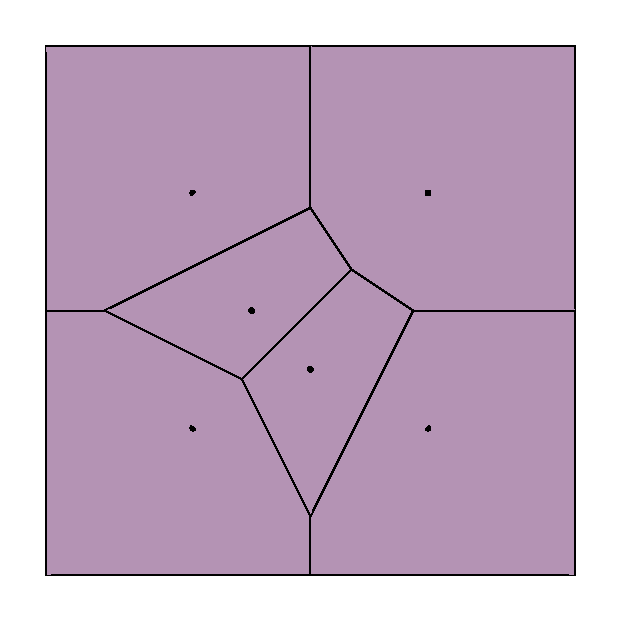
\includegraphics[height=40mm]{vtest_fig_vo}
\end{center}

The set of all Voronoi cells and their faces forms a cell complex.
The vertices of this complex are called the {\em Voronoi vertices\/},
and the extreme rays (i.e. unbounded edges) are  the {\em Voronoi rays\/}.
For each point $v\in R^d$,  the {\em nearest neighbor set\/} 
$nb(S, v)$ of $v$ in $S$ is the set of points $p \in S-v$ which
are closest to $v$ in Euclidean distance.
Alternatively, one can define a point $v \in R^d$ 
to be a {\em Voronoi vertex\/} of $S$ if $nb(S, v)$
is maximal over all nearest neighbor sets.

In order to compute the Voronoi diagram, the following construction
is very important.  For each point $p$ in $S$, consider
the hyperplane tangent to the paraboloid in $R^{d+1}$ at $p$: 
$x_{d+1} = x_1^2 + \cdots + x_d^2$.  This hyperplane is 
represented by $h(p)$: 
\[
\sum_{j=1}^d p_j^2 - \sum_{j=1}^d 2 p_j x_j + x_{d+1} = 0.
\]
By replacing the equality with inequality $\ge$ above for each point $p$,
we obtain the system of $n$ inequalities, which we denote by  
$b - A x \ge 0$.  The polyhedron $P$ in $R^{d+1}$ of all solutions
$x$ to the system of inequalities is a lifting of the Voronoi diagram
to one higher dimensional space.  In other words, by projecting
the polyhedron $P$ onto the original $R^d$ space, we obtain
the Voronoi diagram in the sense that the projection of each facet of $P$
associated with $p \in S$ is exactly the voronoi cell $vo(p)$.
The vertices and the extreme rays of $P$ project exactly to
the Voronoi vertices and the rays, respectively.

\bigskip
\begin{center}
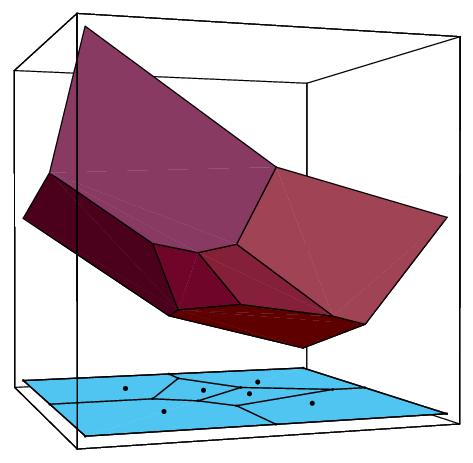
\includegraphics[height=40mm]{vtest_fig_vo3d}
\end{center}

\subsection{What is the Delaunay triangulation in $R^d$? }
\label{voro:dela_def}

See also \ref{voro:def}, \ref{voronoi:complex}.

Let $S$ be a set of $n$ points in $R^d$. 
The convex hull $conv(nb(S, v))$ of the nearest neighbor set of a
Voronoi vertex $v$ is called the Delaunay cell of $v$. 
The Delaunay complex (or triangulation) of $S$
is a partition of the convex hull $conv(S)$ into 
the Delaunay cells of Voronoi vertices together with
their faces.

\bigskip
\begin{center}
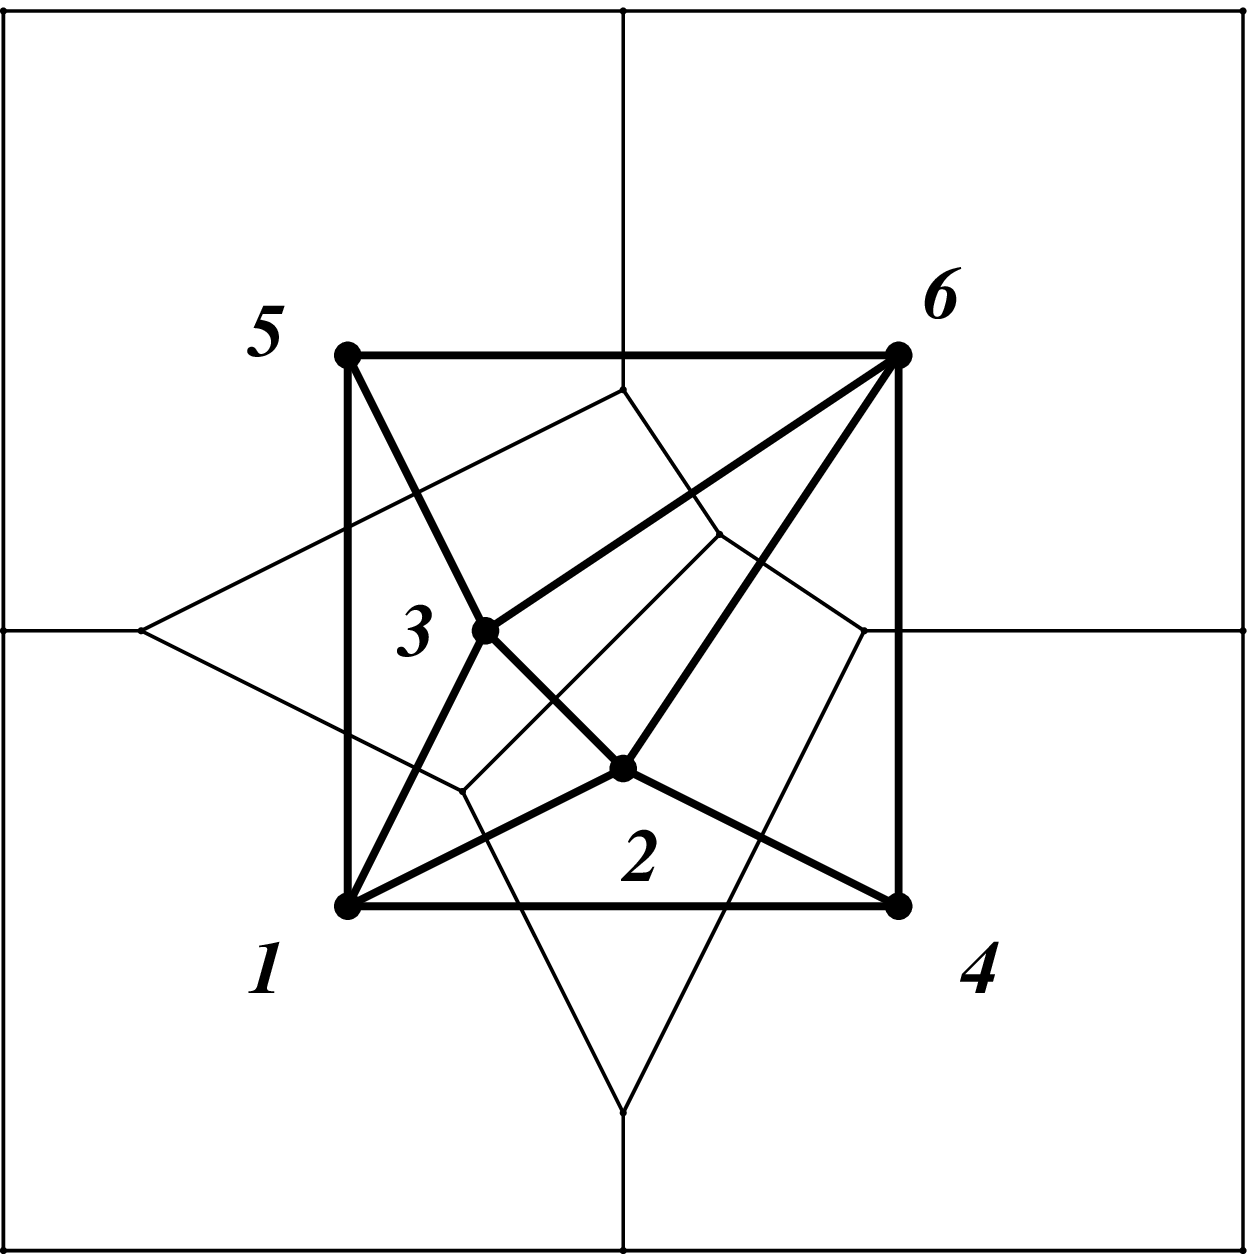
\includegraphics[height=40mm]{vtest_draw_vode}
\end{center}

The Delaunay complex is not in general a triangulation
but becomes a triangulation when the input points are in
{\em general position} (or {\em nondegenerate}),
i.e. no $d+2$ points are cospherical or equivalently there is no
point $c\in R^d$ whose nearest neighbor set has more than $d+1$ elements.

The Delaunay complex is dual to the Voronoi diagram \ref{voro:def}
in the sense that there is a natural bijection between the
two complexes which reverses the face inclusions.

There is a direct way to represent the Delaunay complex, just like
the Voronoi diagram \ref{voro:def}.  In fact, it uses the same 
paraboloid in $R^{d+1}$:  $x_{d+1} = x_1^2 + \cdots + x_d^2$.
Let $f(x) = x_1^2 + \cdots + x_d^2$, and let $\tilde{p}= (p, f(x)) \in R^{d+1}$
for $p \in S$.    Then the so-called lower hull of the lifted points
 $\tilde{S}:=\{\tilde{p}:  p\in S\}$ represents the Delaunay complex.
More precisely, let  
\[
P =  conv(\tilde{S}) + nonneg(e^{d+1})
\]
where $e^{d+1}$ is the unit vector in $R^{d+1}$ whose last component is $1$.
Thus $P$ is the unbounded convex polyhedron
consisting of  $conv(\tilde{S})$ and
any nonnegative shifts by the ``upper'' direction $r$.
The nontrivial claim is that the the boundary complex of $P$ projects
to the Delaunay complex:  any facet of $P$ which is not parallel
to the vertical direction $r$ is a Delaunay cell once its last coordinate
is ignored, and any Delaunay cell is represented this way.

\subsection{Computing the Delaunay complex and the Voronoi diagram.  
What does it mean and how to do it with available software?}
\label{voro:computation}

Let $S$ be a given set of $n$ points in $R^d$.
Computing the Voronoi diagram normally means to generate
the set $Vo(S)$ of Voronoi vertices, and computing the Delaunay complex
is essentially the same thing.  Once the Voronoi vertices are
generated, the nearest neighbor sets $nb(S, v)$ for all Voronoi
vertices $v$ can be easily computed, and in fact most
of the algorithms for generating the Voronoi vertices
computes the nearest neighbor sets as well at the same time.

The complexity of computing the Voronoi diagram is not well
understood in general.   For example, there is no known
algorithm that runs polynomial in the size of input and output.
For the much easier nondegenerate case, there is an algorithm,
known as the reverse search algorithm, which runs
in time $O(n d |Vo(S)|)$.   When the dimension is fixed (in particular
$d=2$), one can analyse complexities of various-type algorithms
in terms of the input size.  In the plane, there are $O(n \log n)$
algorithms that is optimal,
and for fixed $d$ there is an incremental $O(n^{\lceil d/2 \rceil})$ algorithm,
see \cite[Chapter 20]{go-hbdcg-97}.

How large is the number $|Vo(S)|$ of output?  The tight upper bound
was given in \cite{s-eubnf-91} which is 
$O(n^{\left\lfloor (d+1)/2 \right\rfloor})$.
While this bound may be a far over-estimate of expected behavior,
the number of output typically grows exponentially 
in $n$ and $d$, and thus the computation itself
is expected to be heavy.  Therefore, one must take a caution to do
the Delaunay/Voronoi computation.  In fact,
\begin{quote} I know quite a few people who tried to
use Voronoi diagram computation codes in order to accomplish
a much simpler task.
\end{quote}
It is not only a waste of time and computer resources, but
it often leads to a prohibitively hard computation, while
an appropriate use of mathematical techniques resolves
the problem instantly.

For example, the following computations are much simpler
and should be solved via linear programming techniques in Section \ref{Sec:LP}:
\begin{itemize}
\item For given two points $p$ and $q$ in $S$, check whether
their Voronoi cells are adjacent in the Voronoi diagram, see \ref{voro:adjacency}.
\item For any given point $c\in R^d$, find a Delaunay cell
containing $c$, see \ref{dela:cellbylp}.

\end{itemize}

The most natural way to compute the Voronoi diagram is by
computing the vertices and the extreme rays
of the polyhedron in $R^{d+1}$ given
in \ref{voro:def}.  By ignoring the last component
of each vertices we obtain the Voronoi vertices.

\subsubsection{Sample session with cddlib} 
\label{voro:computation:session}

\begin{small}
Consider a simple two dimensional case: $d=2$, $n=6$ and
 $S = \{(0,0), (2,1), (1,2), (4,0), (0,4),(4,4) \}$.  In principle
the session below will work in any $d$ and $n$, although 
the computation time depends heavily on the size.

The first step is to write down the system of linear inequalities
in $(d+1)$ variables as explained in \ref{voro:def}:
for each $p\in S$,
\[
\sum_{j=1}^d p_j^2 - \sum_{j=1}^d 2 p_j x_j + x_{d+1} \ge 0.
\]
For our example, we have:
\[
\begin{array}{rrrr}
  0 &        &        & + x_3 \ge 0\\
  5 & -4 x_1 & -2 x_2 & + x_3 \ge 0\\
  5 & -2 x_1 & -4 x_2 & + x_3 \ge 0\\
 16 & -8 x_1 &        & + x_3 \ge 0\\
 16 &        & -8 x_2 & + x_3 \ge 0\\
 32 & -8 x_1 & -8 x_2 & + x_3 \ge 0
\end{array}
\]


We denote by $P$ the polyhedron of all solutions $x\in R^d$
satisfying the inequalities above.
Now we prepare an input file for cddlib.  The file must 
be in {\em polyhedra\/} format and for the system above,
it is rather straightforward since it essentially
codes the coefficients of the system.

\begin{verbatim}
* filename: vtest_vo.ine
H-representation
begin
 6   4   integer
  0  0  0  1
  5 -4 -2  1
  5 -2 -4  1
 16 -8  0  1
 16  0 -8  1
 32 -8 -8  1
end
incidence
input_adjacency
\end{verbatim}

\noindent
The last two lines ``incidence'' and ``input\_adjacency''
are options for the (old) standalone code cdd+.  They are not necessary
for scdd.c (a sample code for cddlib).   The executables of scdd.c, namely,
scdd (floating-point) or scdd\_gmp (gmp exact rational) computes
the second (generator) representation vtest\_vo.ext of the polyhedron and output
four files vtest\_vo.icd, vtest\_ecd, vo.vtest\_vo.iad, and vtest\_vo.ead.

Now, by running scdd.c with commands:

\begin{verbatim}
% scdd_gmp vtest_vo.ine
\end{verbatim}
or
\begin{verbatim}
% scdd vtest_vo.ine
\end{verbatim}
we obtain the five files mentioned above.  
Among them the most important for our purpose are
the following three, vtest\_vo.ext (all extreme points and rays), 
vtest\_vo.iad (adjacency of facet inequalities) and 
vtest\_vo.ecd (incidence of extreme points/rays and inequalities).  Note
that scdd\_gmp runs in rational exact arithmetic and scdd runs in
floating-point arithmetic.  scdd runs much faster than scdd\_gmp but
it may not give a correct answer.

The file vtest\_vo.ext would be something like the following:

\HTrule
\begin{verbatim}
ext_file: Generators
V-representation
begin
 10 4 rational
 0 -1 0 0
 1 -3/2 2 0
 1 5/6 5/6 0
 1 2 -3/2 0
 0 0 -1 0
 1 27/10 27/10 56/5
 1 15/4 2 14
 0 1 0 8
 0 0 1 8
 1 2 15/4 14
end
\end{verbatim}
\HBrule

The output contains all the vertices
and extreme rays of the (unbounded) polyhedron $P$ in $R^3$.
Namely each row starting with ``1'' represents a vertex.
So the second row 
\begin{verbatim}  1 -3/2 2 0\end{verbatim}
represents the vertex $(-3/2, 2, 0)$.  Each row starting
with ``0'' represents an extreme ray, e.g. the first row
\begin{verbatim}  0 -1 0 0 \end{verbatim}
represents the ray  $(-1, 0, 0)$.

By ignoring the last components, we obtain the set of six
Voronoi vertices $(-3/2, 2)$, $(5/6, 5/6)$, $(2, -3/2)$, $(27/10, 27/10)$,
$(15/4, 2)$ and $(2, 15/4)$ and four Voronoi rays
$(-1, 0)$, $(0, -1)$, $(1, 0)$ and $(0, 1)$.

The incidence file vtest\_vo.ecd file:

\HTrule
\begin{verbatim}
ecd_file: Incidence of generators and inequalities
begin
  10    7
 1 3 : 1 5 7 
 2 3 : 1 3 5 
 3 3 : 1 2 3 
 4 3 : 1 2 4 
 5 3 : 1 4 7 
 6 3 : 2 3 6 
 7 3 : 2 4 6 
 8 3 : 4 6 7 
 9 3 : 5 6 7 
 10 3 : 3 5 6 
end
\end{verbatim}
\HBrule

Each row corresponds to the same row in vtest\_vo.ext file.
For example, the second data 
\begin{verbatim} 2 3 : 1 3 5\end{verbatim}
says the second data in vtest\_vo.ext file:
\begin{verbatim} 1 -3/2 2 0  
\end{verbatim}
is a voronoi vertex whose nearest neighbor set
is $\{p^1, p^3, p^5\}$.  Also, this set corresponds
to a Delaunay cell.
Similarly, the first row
\begin{verbatim} 1 3 : 1 5 7\end{verbatim}
indicates the ray (the first output in vtest\_vo.ext file)
\begin{verbatim}  0 -1 0 0 \end{verbatim}
is determined by 1, 5 and 7th halfspaces.  The 7th halfspace
is an artificial one corresponding to the infinity.  So this ray
is determined by the input points 1 and 5 and going to infinity.

Thus, the index sets (triples, in this case) not containing
the infinity $7$ determine all Delaunay cells, and those
containing $7$ correspond to the Voronoi rays.

Finally, look at the vtest\_vo.iad file:
 
 
\HTrule
\begin{verbatim}
iad_file: Adjacency of inequalities
begin
  7    7
 1 -5 : 1 6 
 2 -4 : 2 5 7 
 3 -4 : 3 4 7 
 4 -4 : 3 4 5 
 5 -4 : 2 4 5 
 6 -5 : 1 6 
 7 -4 : 2 3 7 
end
\end{verbatim}
\HBrule

\noindent
This file contains the graph structure (adjacency list) of the Delaunay complex
and equivalently the adjacency of Voronoi cells in the Voronoi
diagram.

\bigskip
\begin{center}
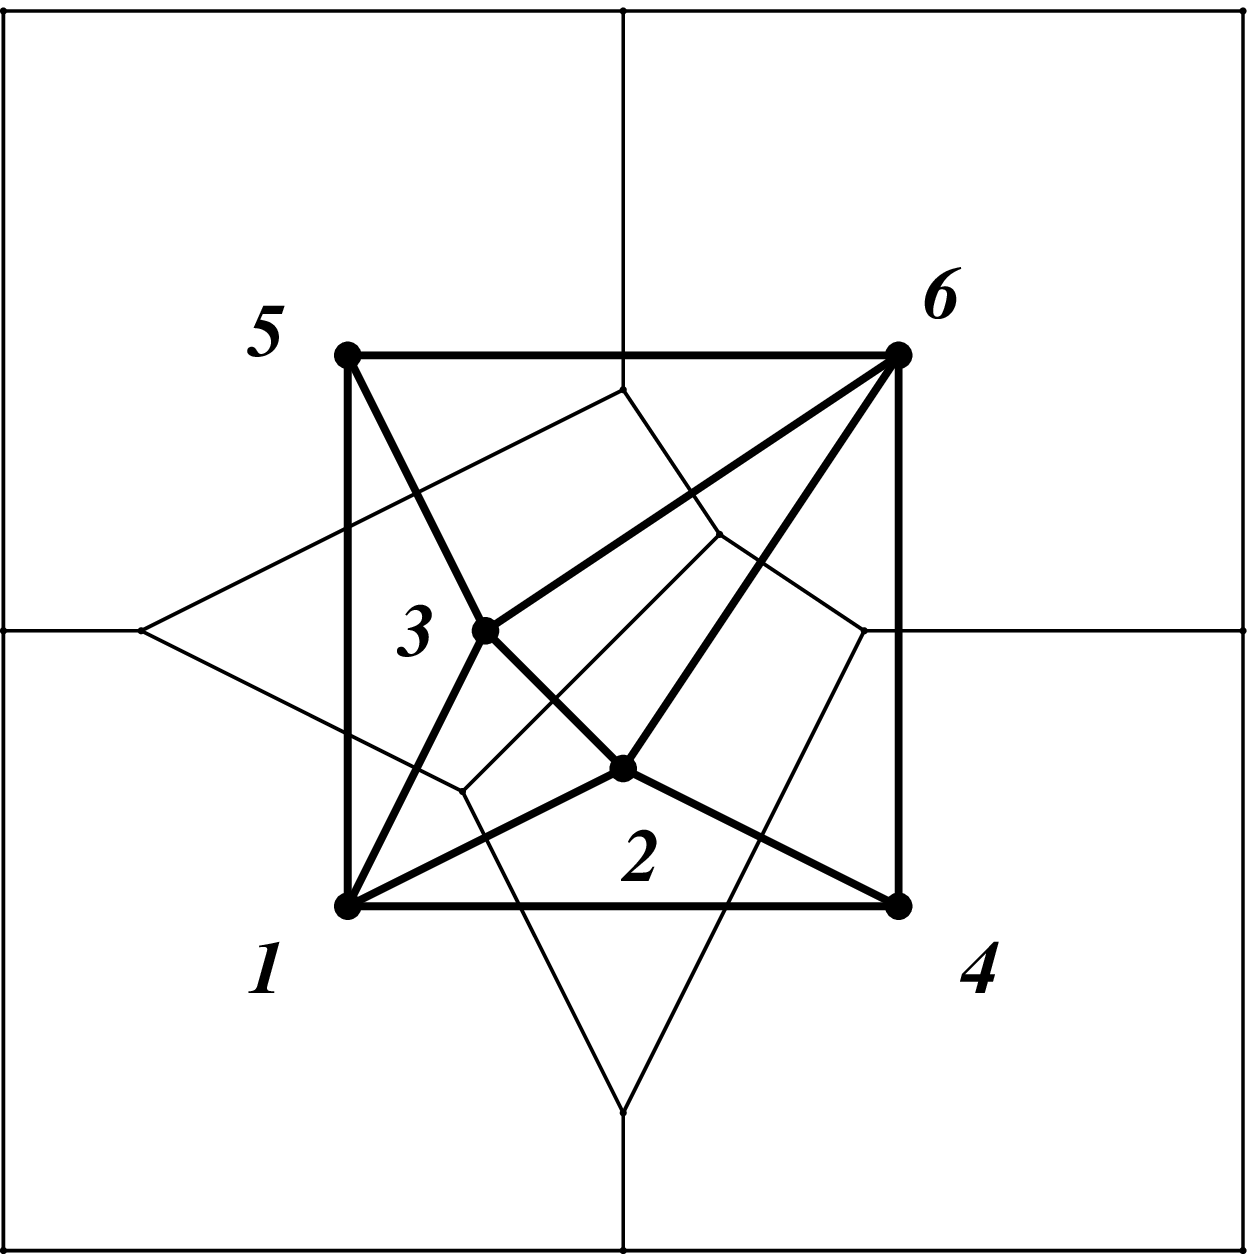
\includegraphics[height=40mm]{vtest_draw_vode}
\end{center}

\noindent
For example, the first row
\begin{verbatim}
  1 -5 : 1 6 
\end{verbatim}
says that the first Voronoi cell is adjacent to $5$ cells.
The row is equivalent to
\begin{verbatim}
  1 5 : 2 3 4 5 7
\end{verbatim}
Notice that the cddlib lists the non-neighbors whenever
the number of non-neighbors is smaller than that of neighbors.  
Thus, the negative
$-5$ indicates that the list is non-neighbors.

In the language of the Delaunay complex, the first line in this file
says the point $p^1$ is adjacent to $5$ neighbors
$p^2$, $p^3$, $p^4$, $p^5$ and $p^7$.  Here,
the point $p^7$ is the artificial infinity point
which is considered adjacent to any input point
whose Voronoi cell is unbounded.

As we remarked before, this graph information can be
computed much more efficiently by linear programming.
See \ref{voro:adjacency}.
\end{small}

\subsection{Is it possible to compute only the adjacencies of Voronoi cells in
the Voronoi diagram efficiently?}
\label{voro:adjacency}

Yes, it can be done very efficiently by linear programming (LP), and
very importantly this can be done for very large scale problems,
with practically no bounds on the size with an efficient LP solver.

The method is simple.  The lifting technique we described in
\ref{voro:def} immediately gives the idea.  Recall that
the Voronoi diagram
of a set $S$ of $n$ points in $R^d$
 is the projection of the following $(d+1)$-polyhedron to
$R^d$ space of the first $d$ components.
\[
P = \{ x\in R^{d+1} \; | \;  \sum_{j=1}^d p_j^2 - \sum_{j=1}^d 2 p_j x_j + x_{d+1} \ge 0
  \quad \forall p \in S \}.
\]
For simplicity, denote it as
\[
P = \{ x\in R^{d+1} \; | \;  b - A x \ge 0 \},
\]
where $A$ is a given $n \times (d+1)$ matrix and $b$ is a $n$-vector.
Now for each $i=1,\ldots, n$, consider the $i$th facet $F_i$ of $P$:
\begin{align} \label{eq:voro_facet}
F_i = \{ x\in R^{d+1} \; | \;  b - A\; x \ge 0 \mbox{ and }
 b_i - A_i \; x \le 0 \},
\end{align} 
Two facets $F_i$ and $F_j$ are called {\em adjacent\/} if 
the intersection $F_i \cap F_j$ is a facet of both, i.e.
has dimension $d-2$. An equivalent definition is: they are
{\em adjacent\/} if (*) the facet $F_i$ becomes larger once the
facet $F_j$ is removed from the polyhedron, i.e. the $j$th
inequality is removed from the system $b - A \; x \ge 0$. 

It is easy to see that two Voronoi cells $vo(p^i)$ and $vo(p^j)$
are adjacent if and only if the corresponding facets $F_i$ and
$F_j$ are adjacent in the polyhedron $P$.
Now, we formulate the following LP for any
distinct $i$, $j = 1,2, \ldots,n$:

\begin{align} \label{eq:voro_facet_lp}
\begin{array}{lllllll}
&\text{minimize}    & \quad f(x) :=  & b_j & - &  A_j & x  \\
&\text{subject to}  &                & b'  & - &  A & x \; \ge \; 0 \\  
&                   &                & b_i & - &  A_i & x \; \le \; 0,
\end{array}
\end{align}

\noindent
where $b'$ is equal to $b$ except for $j$th component
$b'_j = b_j + 1$.  The new inequality system  $b' - A \; x \ge 0$
is simply a modification of the original system 
obtained by relaxing the $j$th inequality a little bit.
An important remark is, by definition (*), $F_j$ and $F_i$
are adjacent if and only if the objective value $f(x)$
is negative at an optimum solution.  Thus we formulated
the Voronoi adjacency computation as an LP problem.

How much do we gain by using LP for the adjacency computation, instead
of computing the whole Voronoi diagram?
A lot.   It is hard to exaggerate this, because the LP (\ref{eq:voro_facet_lp})
(in fact any LP) is solvable in polynomial time, 
whereas the associated Voronoi computation is exponential in
$d$ and $n$.  Using the standard simplex method, the time complexity of solving
an LP is not polynomial, but the practical complexity is roughly
$O(n  d^3)$.

\subsubsection{Sample session with cddlib}
\label{voro:adjacency:session}
\begin{small}
With cddlib, a setup for computing the adjacency of Voronoi cells is
quite simple.  Consider the same example
\ref{voro:computation:session}.  For each input point
$i=1,2,3,4,5,6$, we write the inequality system for the facet $F_i$:
\[
\begin{array}{ll}
& b -  A  x \ge 0 \text{ and }\\
& b_i -  A_i x \le 0 \text{,}
\end{array}
\]
instead of writing the relaxed inequality (\ref{eq:voro_facet_lp}).  
For example, for $i=4$, we have

\HTrule
\begin{verbatim}
H-representation
begin
 7   4   real
  0  0  0  1
  5 -4 -2  1
  5 -2 -4  1
 16 -8  0  1
 16  0 -8  1
 32 -8 -8  1
-16  8  0 -1
end
facet_listing
\end{verbatim}
\HBrule

\noindent
We save this as the file vtest\_vof4.ine
The last inequality is the negative of the forth inequality
to force the forth inequality to be equality.

The old code cdd+ accepts an option called ``facet\_listing''.  With
this option, cdd+ will check which of
the given inequalities is redundant or not (essential), by solving
the associated LP's  (\ref{eq:voro_facet_lp}) 
for each inequality $j$.

With cddlib,  we can do the same test by 
the program redcheck.c, which is distributed in
the src subdirectory.   This program ignores this option line, and
does the redundancy removal and finds a minimal representation of the polyhedron.

By running the executable  redcheck\_gmp (exact gmp rational) or redcheck (floating-point) by 

\begin{verbatim}
% redcheck_gmp vtest_vof4.ine
\end{verbatim}
we will get the output:

\HTrule
\begin{verbatim}
input file vtest_vof4.ine is open
Canonicalize the matrix.
Implicit linearity rows are: 4 7 

Redundant rows are: 3 5 

Nonredundant representation:
The new row positions are as follows (orig:new).
Each redundant row has the new number 0.
Each deleted duplicated row has a number nagative of the row that
represents its equivalence class.
 1:2 2:3 3:0 4:1 5:0 6:4 7:0
H-representation
linearity 1  1
begin
 4 4 rational
 16 -8 0 1
 0 0 0 1
 5 -4 -2 1
 32 -8 -8 1
end
\end{verbatim}
\HBrule

First of all, it recognizes that the $4$th and the $7$th row
are implicit equations and should be written as an equation.
Then, the redundant rows are recognized as $3$rd and $5$th.  Thus, we can
consider the set $\{1, 2, 6\}$ as the indices of essential constraints, or
equivalently the indices of Voronoi cells adjacent to the $4$th
cell.  Of course, this adjacency coincides with the adjacency
of input points in the Delaunay triangulation.
See the figure below.

\bigskip
\begin{center}
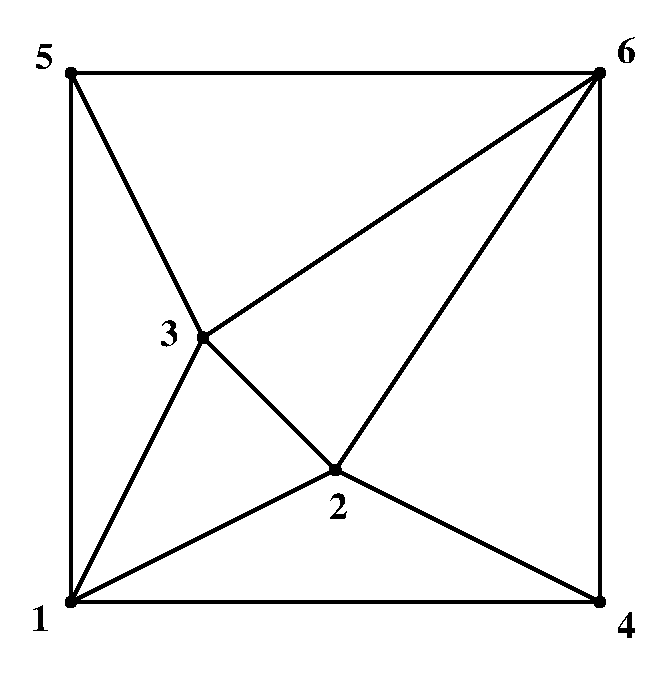
\includegraphics[height=40mm]{vtest_draw_de}
\end{center}


\end{small}

\subsection{Is it possible to compute only the edges of the Delaunay complex
(triangulation) ?} \label{voro:de_adjacency}

This is essentially the same question as computing
the adjacencies of Voronoi cells, see \ref{voro:adjacency}.

\subsection{Is it possible to determine the Delaunay cell containing
a given point efficiently?}
\label{dela:cellbylp}

Yes, it is possible to find the nearest point set associated
with the Delaunay cell containing a given point $c\in R^d$.
As we discussed in Section \ref{voro:dela_def}, the Delaunay
complex can be represented by the convex hull of appropriately
lifted points in $R^{d+1}$, and the non-vertical facets coincide with
the Delaunay cells once they are projected to the original space.
Thus the problem of determining the Delaunay cell containing a given
point $c$ can be reduced to finding the first facet of a polyhedron
``shoot'' by a ray.

To be more precise, let 
$f(x) = x_1^2 + \cdots + x_d^2$, and let $\tilde{p}= (p, f(x)) \in R^{d+1}$
for $p \in S$.    Then the lower hull $P$ of the lifted points
 $\tilde{S}:=\{\tilde{p}:  p\in S\}$:
\[
P =  conv(\tilde{S}) + nonneg(e^{d+1})
\]
represents the Delaunay complex. 
Here $e^{d+1}$ is the unit vetor in $R^{d+1}$ whose last component is $1$.
For any vector $\tilde{y} \in R^{d+1}$ and $y_0 \in R$, 
let $\tilde{y}^T x \ge -y_0$ denote a general inequality of a variable
vector $x \in R^{d+1}$.  For such an inequality
to represent a valid inequality of $P$ (see Section \ref{polytope:faces}), 
it must be satisfied by all points in $\tilde{S}$:
\begin{equation} \label{voro:delfacet1}
 \tilde{y}^T \tilde{p} \ge -y_0, \forall \tilde{p} \in \tilde{S},
\end{equation}
and by any points shifted vertically upwards, i.e.
\[
 \tilde{y}^T ( \tilde{p} + \alpha e^{d+1})
\ge -y_0, \forall \tilde{p} \in \tilde{S} \text{ and any } \alpha \ge 0.
\]
\noindent
Under the first inequality (\ref{voro:delfacet1}), 
the last inequality is equivalent to 
\begin{equation} \label{voro:delfacet2}
 \tilde{y}_{d+1} \ge 0.
\end{equation}

\noindent
Now every Delaunay cell
is a projection of a non-vertical facet of $P$.  We are thus looking
for an inequality $\tilde{y}^T x \ge -y_0$ satisfying
(\ref{voro:delfacet1}), (\ref{voro:delfacet2}) and $y_{d+1}\neq 0$.
By scaling with $\tilde{y}_{d+1}>0$, we may assume $\tilde{y}_{d+1} = 1$.
For a given point $c$, let $\tilde{c} = (c, 0)^T$, and let
$L(\lambda)= \tilde{c} + \lambda \; e^{d+1}$, $\lambda \ge 0$.
Determining the Delaunay cell containing $c$
is equivalent to finding the last inequality ``hit'' by the halfline
$L$.  More precisely, it is to find a non-vertical facet inequality
such that the intersecion point of the corresponding hyperplane
$\{ x :  y^T x = -y_0\}$ and the half line $L(\lambda), \lambda \ge 0$
is highest possible.  

By substituting $L(\lambda)$ for $x$ in $y^T x = -y_0$ with
$\tilde{y}_{d+1} = 1$, we obtain
\[
 \lambda = -y_0 - y^T c,
\]
where $y$ denotes the vector $\tilde{y}$ without the last coordinate
$\tilde{y}_{d+1}$.  The LP formulation is therefore:
\begin{alignat}{3} \label{eq:dela_celllp}
&\text{minimize}  
  &  z :=  &       &   y_0 + & y^T c \\
&\text{subject to}  
  &        & f(p) & + y_0 +  &y^T p \ge 0 \text{ for all }  p \in S.  \nonumber
\end{alignat}
While an optimal solution $(y_0, y)$ to this LP may not determine
any facet in general, the simplex method always returns an optimal
basic solution which determines a facet inequality in this case.
The Delaunay cell containing $c$ is the one determined by 
the set of points in $S$ whose corresponding inequalities
are satisfied by equality at the optimal solution.  If the LP
solution is not degenerate, the dual variables that are positive
at the dual optimal solution coincides with the former set.

It is important to note that the above LP might be unbounded.  If it
is unbounded, it can be easily shown that $c$ is not in
any Delaunay cell, i.e., not in the convex hull of $S$.  A certificate
of unboundedness actually induces a hyperplane strongly separating
$c$ from $S$. (why?)

\subsubsection{Sample session with cddlib} 
\label{dela:computation:session}

\begin{small}

With cddlib (scdd.c) and any reasonable LP code, the only necessary step should be
to prepare the LP file for determination
of the Delaunay cell containing a given point $c\in R^d$.  
Consider the same example \ref{voro:computation:session}.  

For a given point $c = (3, 2)$, 
the LP (\ref{eq:dela_celllp}) file for scdd or scdd\_gmp is

\HTrule
\begin{verbatim}
H-representation
begin
  6  4  rational
  0  1  0  0
  5  1  2  1
  5  1  1  2
 16  1  4  0
 16  1  0  4
 32  1  4  4
end
minimize
  0  1  3  2
\end{verbatim}
\HBrule

\noindent
The solution by scdd\_gmp is:

\HTrule
\begin{verbatim}
* #constraints = 6
* #variables   = 3
* Algorithm: dual simplex algorithm
* minimization is chosen
* Objective function is
 0 + 1 X[  1] + 3 X[  2] + 2 X[  3]
* LP status: a dual pair (x,y) of optimal solutions found.
begin
  primal_solution
    1 :  14
    2 :  -15/2
    3 :  -4
  dual_solution
    2 :  -1/2
    4 :  -1/8
    6 :  -3/8
  optimal_value :  -33/2
end
\end{verbatim}
\HBrule

Therefore, the facet inequality is $ 14 - 15/2 x_1 - 4 x_2 \ge 0$, and
the dual solution indicates that the points $p^2, p^4, p^6$ determine
the Delaunay cell which contains $(3, 2)$.


\end{small}



\subsection{What is the best upper bound of the numbers of 
simplices in the Delaunay triangulation?} \label{voro:upperbound}

See  \ref{voro:computation}.

% --------------------- Linear Programming --------------------

\section{Linear Programming} \label{Sec:LP}

\subsection{What is LP?} \label{LP:def}

A linear programming (abbreviated by LP) is to find a maximizer or
minimizer of a linear function subject to linear inequality constraints.
More precisely, 

\begin{alignat}{2}
&\text{maximize}  
  & \quad f(x) :=  & \sum_{j=1}^d c_j x_j   \label{eq:LP} \\
&\text{subject to}  
  &                & \sum_{j=1}^{d}  a_{ij} x_j \le b_i \text{ for all }  i=1,2,\ldots, m, \\  \nonumber
\end{alignat}
where $A=[a_{ij}]$ is a given rational $m\times d$ matrix, 
$c=[c_j] $ and $b=[b_i]$ are given rational $d$- and $n$-vector.
We often write an LP in matrix form:
\begin{alignat}{2}
&\text{maximize} 
  & \quad f(x) :=  & c^T x   \label{eq:LPmat} \\
&\text{subject to}  
  &                        & A  x \le b. \\  \nonumber
\end{alignat}

Theoretically every rational
LP is solvable in polynomial time by both the ellipsoid method of Khachian
(see \cite{k-palp-79,s-tlip-86})
various interior point methods (see \cite{k-nptal-84,rtv-talpip-97}).
The well-known simplex method of Dantzig (see \cite{d-lpe-63,c-lp-83})
has no known polynomial variants.  In practice,
very large LPs can be solved efficiently 
by both the simplex method and interior-point
methods.  
For example, it is very easy on a standard unix station to solve an LP with
$d=100$ and $m=100,000$, while the vertex enumeration/convex hull
computation of the same size is simply intractable.
There are many commercial codes and public codes available.
See the LP FAQ \cite{fg-lpfaq}.  Two excellent classical books on LP are
Chvatal's textbook \cite{c-lp-83} and Schrijver's 
``researcher's bible'' \cite{s-tlip-86}.

There is a new textbook on LP theory and Optimization \cite{f-io-20} which explains the duality
theory and the finite pivoting theory quite differently from the classical
textbooks.   One essential difference comes from a rather elementary fact
that the classical numbering of the dual
variables is not mathematically sound, see \cite[Chap 1--4]{f-io-20}.  Once
the dual variables are properly renumbered, one can see that the LP duality
 is a property of the orthogonal dual pairs of vector subspaces
of $R^n$.


% ------------------------------ Codes ----------------------------------
\section{Polyhedral Computation Codes} \label{Sec:codes}
\begin{itemize}
\item cddlib, cdd  and cdd+ \cite{f-cddhome} 
(C and C++ implementations of the double description method \cite{mrtt-ddm-53}).
\begin{quote}
Comments: Runs on both floating and exact arithmetic.  Efficient for highly 
degenerate cases.  The exact
versions are much slower.   It can remove redundancies from input data
using a built-in LP code.  cddlib is a C-library with basic
polyhedral conversion functions and LP solvers.  cddlib can be
compiled with both GMP rational (mpq) and floating point arithmetic.
A new arithmetic (with an arithmetic library) can be added to cddlib.
\end{quote}

\item lrs and lrslib  \cite{a-lrshome-01} (C implementation of the reverse search algorithm 
\cite{af-pachv-92}).  A parallel version prs was developed by A. Marzetta,
see \cite{bmfn-psbza-96}.
\begin{quote}
Comments: Exact arithmetic only, efficient for nondegenerate cases.  Uses a little memory
and perhaps the only available code which can deal with problems in high dimensions, say, over $20$.  
There is a parallel implementation mplrs that uses the MPI library.
\end{quote}

\item pd  \cite{m-pdcip-97} (C implementation of the primal-dual algorithm 
\cite{bfm-pdmvf-97}). 
\begin{quote}
Comments: Exact arithmetic only, efficient for dually nondegenerate cases. 
\end{quote}

\item qhull \cite{bdh-qach-96,bdh-qach-03} (C implementation of
the beneath-beyond method, see \cite{e-acg-87,m-cg-94},
which is a sort of dual of the double description method). 
\begin{quote}
Comments: Floating arithmetic only but handles numerical problems
well.  Highly efficient for nondegenerate cases.   
User can call it as a C-libary.
\end{quote}

\item porta \cite{cl-porta-97} (C implementation of
the Fourier-Motzkin elimination method \cite{z-lop-94}). 

\begin{quote}
Comments: Efficient for combinatorial (e.g. 0-1) polytopes.
Guarantees correct numerical results as long as
double precision integer arithmetic does not overflow.
It can list all integer solutions in a polytope.
\end{quote}

\item polymake \cite{gj-pm-99} (computational
environment for the algorithmic 
treatment of polytopes and polyhedra). 

\begin{quote}
One can generate convex polytopes and do various computations
with convex polyhedra.  
It uses cddlib/porta/lrslib for representation conversions. 
It is extendable by writing own "rules" to generate
new structures/data associated with polyhedra.
\end{quote}


\item PPL  \cite{b-pplhome} (C++ implementation of the double description method \cite{mrtt-ddm-53}). 
\begin{quote}
Comments: A modern efficient implementation.  Exact arithmetic only.
\end{quote}

\item zeRone \cite{l-zvefzo-99} (C implementation of
the backtrack vertex enumeration algorithm for
0-1 H-polytopes \cite{bl-vs01ps-98}. 

\begin{quote}
Comments: In general, the straightforward backtrack algorithm
for the vertex enumeration problem must solve NP-complete
decision problems, as it was shown in \cite{flm-abala-97}.
The situation is different for 0-1 polytopes and 
the problem is strongly polynomially solvable.  The code
can generate all 0-1 points in a general H-polytope.
It relies on the commercial LP solver CPLEX.
\end{quote}


\item Pointers to many other programs in geometric computations 
are stored in \cite{a-dcg,e-cgp}. 

\item For linear programming, one should check the Linear Programming
FAQ at \cite{fg-lpfaq}.  It lists both public (open source) and commercial
codes.

\end{itemize}

\section{Acknowledgements}
The author expresses his sincere thanks to Dr. Vera Rosta who
read an earlier version of FAQ carefully, found numerous errors
and provided with many helpful suggestions.


\addtolength{\baselineskip}{-0.3\baselineskip}
\bibliographystyle{alpha}

\bibliography{fukuda1,fukuda2}


\end{document}

